{
\metroset{titleformat frame=smallcaps}
\begin{frame}{Use Case 1: Smart Congestion Control}
\vspace{6pt}
  \subtitlebar{Reinforcement Learning + INT telemetry for proactive traffic management}

  \begin{columns}[T, totalwidth=\textwidth]

    % ── Left: 3 Boxes ─────────────────────────────────────
    \begin{column}{0.44\textwidth}

      \begin{tcolorbox}[problemcard=problemred]
        {\color{problemred}\bfseries\scriptsize The Problem}\\[2pt]
        {\footnotesize\color{HUAdark}
          Traditional networks rely on static paths,
          causing bottlenecks during sudden traffic
          bursts (\textit{Elephant Flows}).}
      \end{tcolorbox}

      \vspace{4pt}

      \begin{tcolorbox}[problemcard=HUAblue]
        {\color{HUAblue}\bfseries\scriptsize AI in Action}\\[2pt]
        {\footnotesize\color{HUAdark}
          A Reinforcement Learning model monitors
          link and node load via INT telemetry,
          and adjusts routing rules in real time.}
      \end{tcolorbox}

      \vspace{4pt}

      \begin{tcolorbox}[problemcard=solutiongreen]
        {\color{solutiongreen}\bfseries\scriptsize Result}\\[2pt]
        {\footnotesize\color{HUAdark}
          Optimal routing rules applied at wire-speed ---
          maximizing bandwidth and preventing
          congestion proactively.}
      \end{tcolorbox}

    \end{column}

    % ── Vertical Divider ─────────────────────────────────
    \begin{column}{0.02\textwidth}
      \centering
      \textcolor{HUAlight}{\rule{0.5pt}{0.80\textheight}}
    \end{column}

    % ── Right: Fig. 10 ───────────────────────────────────
    \begin{column}{0.45\textwidth}
      \centering
      \vspace{0.15cm}
      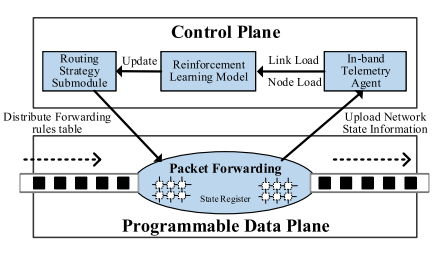
\includegraphics[width=\textwidth]{figures/fig10.png}
      \vspace{0.15cm}
      \begin{tcolorbox}[
        enhanced, boxrule=0pt,
        colback=HUApale, colframe=HUApale,
        arc=3pt, left=5pt, right=5pt,
        top=2pt, bottom=2pt,
      ]
        \centering
        \scriptsize\color{HUAdark}\itshape
        Framework of Network Congestion Control
        %(Quan et al., Fig.~10)
      \end{tcolorbox}
    \end{column}

  \end{columns}

\end{frame}
}